\section{International Agreements Datasets}

To investigate to what extent the COVID-19 pandemic will help countries to reach the goals of the international agreements such as the \textit{Paris Agreement under the United Nations Framework Convention on Climate Change}, we needed to find and understand the goals of such agreements. Specifically, we took a closer look at the Paris Agreement and the agreements of the EU. When we researched the agreements of the EU members, we found out that these agreements are incorporated in the Paris agreement. Thus, we focused on gathering data about the Paris Agreement and handle two international agreements at a time.

\subsection{How Does the Paris Agreement Work?}

Basically, the \textit{Paris Agreement} states that every country  ratifying the treaty acknowledges anthropogenic climate change, commits to the well below \SI{2}{\degreeCelsius} and further aims to limit global warming to \SI{1.5}{\degreeCelsius}. To reach these goals, every country has to define its contribution to fight climate change by itself. These so-called \textbf{n}ationally \textbf{d}etermined \textbf{c}ontributions (NDCs) have to be submitted every five years with new, even stricter goals. Furthermore, countries are also allowed to define the same goals in a group, as for example the member of the EU did.

\subsection{Gathering and Pre-processing Data}

The great challenge in finding data about each country's goals, is that every country defines their own goals, without a greater frame. Thus, countries can for example define a cut in greenhouse gas emissions given as a percentage referring to the emissions in a certain year. It is also possible to state a total amount of greenhouse gases a country wants to reduce its emissions. Also, in some NDCs, countries state that they will build more climate-friendly energy plants. Other, mainly less industrialized countries had a mix of unconditioned and conditioned goals. From these few examples, we can already deduce that the data we can gather from the NDCs is highly non-uniform.

Additionally, there is no readily available data about the NDCs. This means, our team would have to read through every NDC and extract the relevant information by hand, consuming an incredible amount of manpower. Luckily, we found a website\footnote{See \url{https://www.carbonbrief.org/paris-2015-tracking-country-climate-pledges}}, in which  all NDCs are summarized to the very core of information. From this, we started to extract the  designated reduction in greenhouse gas emissions for several countries. However, we quickly realized that this would still consume too much man power. Therefore, we decided to only take a closer look at the eight largest contributors, covering more than 70\% of the worlds greenhouse gas emissions in 2017.\footnote{See \url{https://www.worldometers.info/co2-emissions/}} These contributors are China, the US, the EU, India, Brazil, Russia, Japan and Canada in descending order.

Most of the contributors we considered stated a range of emission reduction they aim for. To compare the data more easily, we simply took the mean of minimum and maximum percentage of emission reduction in these cases. Apart from that, the data is rather uniform and we thus did not have to  pre-process it any more. To the data we had from the website\footnote{See \url{https://www.carbonbrief.org/paris-2015-tracking-country-climate-pledges}}, we added the share of \ce{CO2}  emissions in 2012 and 2017 and the total \ce{CO2}  emissions in the referenced year.

\subsection{Data and Plots}

\begin{table}[htb]
	\begin{center}
		\begin{tabular}{lrrrr}
			Country & Share of \ce{CO2} Emissions [\%] & Reduction Goal [\%] & Compared to Year & Fulfill by Year \\\midrule
			China & 24.48 & *62.5 & 2005 & 2030\\
			USA & 13.63 & *27 & 2005 & 2025\\
			EU & 10.94 & 40 & 1990 & 2030\\
			India & 7.18 & *34 & 2005 & 2030\\
			Russia & 4.48 & *27.5 & 2005 & 2025\\
			Japan & 3.35 & 26 & 1990 & 2030\\
			Canada & 1.76 & 30 & 2013 & 2030\\
			Brazil & 1.68 & 37 & 2005 & 2030\\
		\end{tabular}
		\caption{Countries are in descending order by their respective share in global \ce{CO2} emissions in 2017. Greenhouse gas emission reduction goals with an asterisk * are mean values of the range of maximum and minimum reduction goal of the respective country. Further, the year every country refers its reduction goal to and the year by that each country wants to reach its goal is given.}
		\label{tab:data_co2goals}
	\end{center}
	
\end{table}

In \autoref{tab:data_co2goals} we summarized the most important part of the data we gathered for the greenhouse gas emission reduction goals. With this data, we created the plots in \autoref{fig:co2goals_line} and \autoref{fig:co2goals_bubble}. In \autoref{fig:co2goals_line} we simply draw a line from the starting point to the goal of each country. The starting point is at the year each country refers to in its goals, the value is thus set to \SI{100}{\percent} for every respective country. The end point is at the year every country wants to achieve its goals at the height \SI{100}{\percent} minus the reduction goal. The height therefore corresponds to the greenhouse gas emission level each country wants to achieve in the respective year, compared to the year it referred to. From the slopes, we can deduce the rate of greenhouse gas emission reduction in \%/year. This can be used as a measure of how ambitious each country is.

To put the ambitions of each country into perspective, we also need to consider its contribution to the global greenhouse gas emissions. We visualized this in \autoref{fig:co2goals_bubble}, a bubble plot  where the size of each bubble represents the country's share of greenhouse gas emissions. The black line represents the lower boundary of emission reductions to reach the \SI{1.5}{\degreeCelsius} goal\footnote{We need to cut emissions by 45\% by 2030, see \url{https://www.scientificamerican.com/article/global-promises-to-reduce-co2-are-falling-short-of-1-5-degree-c-warming-goal/}}. As we see, only China's goals are ambitious enough to actually reach the \SI{1.5}{\degreeCelsius} goal all countries aim for. Still, the US, the EU and Russia ratified goals that are at least close to the \SI{1.5}{\degreeCelsius} goal. Other countries are less ambitious.

%old plots, not as subplots
%\begin{figure}[htb]
%	\begin{center}
%		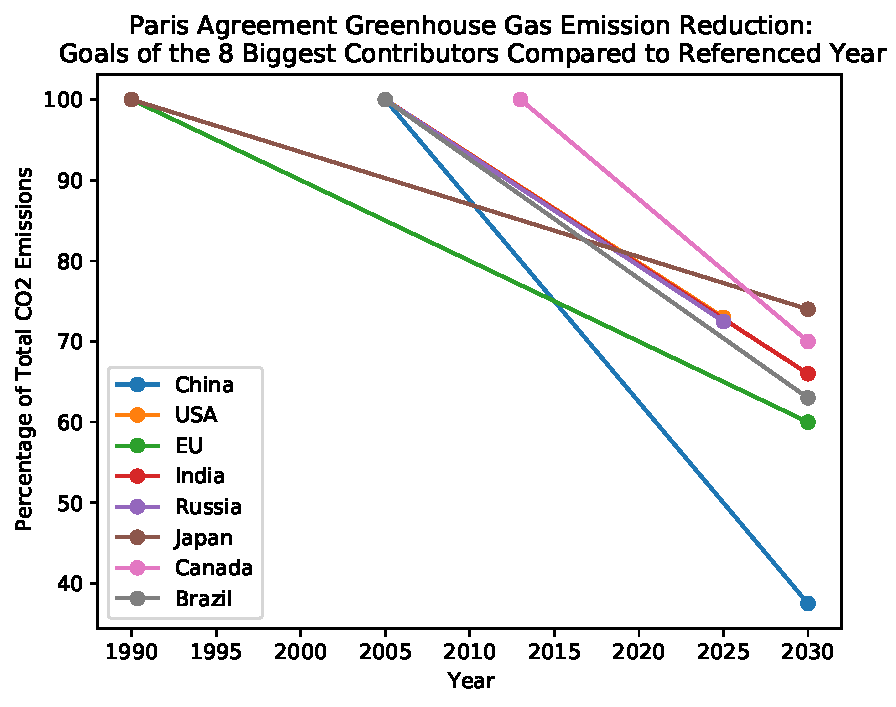
\includegraphics[width=0.8\textwidth]{co2goals/co2goals_lines.pdf}
%		\caption{Line plot for each country's goal compared to the reference year. The $y$-axis represents the greenhouse gas emissions of each country in percent, the $x$-axis the year. Each line starts at (referred  year, 1) and ends at (\(1-\)goal, targeted year). The slopes thus represent the rate of reduction per year in \%/year. This plot does not state anything about absolute data or the contribution of the countries to global greenhouse gas emissions however.}
%		\label{fig:co2goals_line}
%	\end{center}
%\end{figure}
%
%\begin{figure}[htb]
%	\begin{center}
%		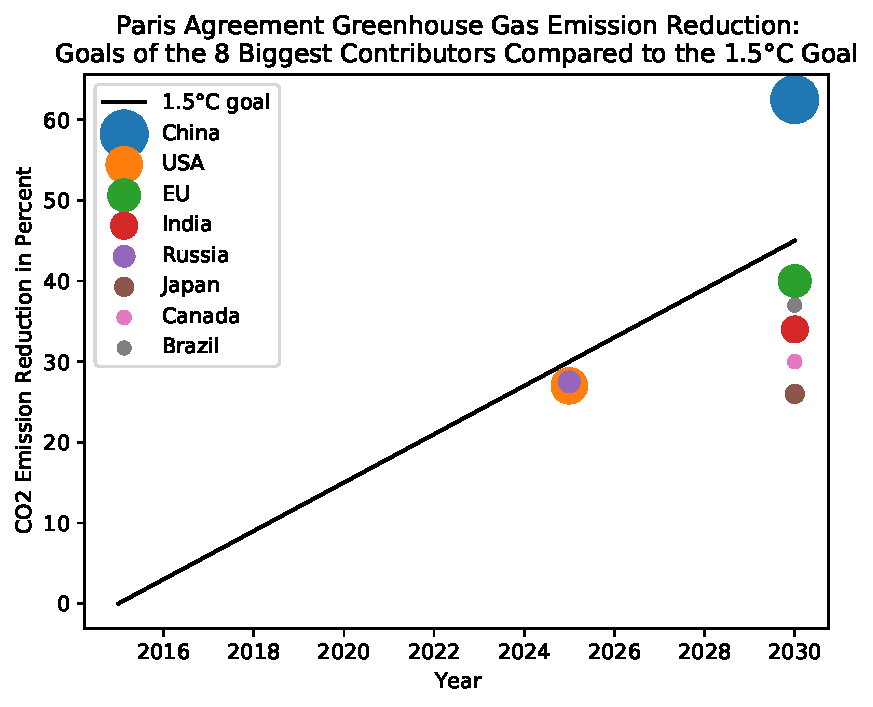
\includegraphics[width=0.8\textwidth]{co2goals/co2goals_bubbles.pdf}
%		\caption{Bubble plot that visualizes how ambitious each country is. The $y$-axis represents the greenhouse gas emission reduction goal in percent, the $x$-axis the year. The size of each bubble corresponds to its share in global greenhouse gas emissions. The black line gives the necessary emission reductions to reach the \SI{1.5}{\degreeCelsius} goal.}
%		\label{fig:co2goals_bubble}
%	\end{center}
%\end{figure}


%\begin{figure}[htb]
%	\begin{center}
%		\begin{subfigure}[b]{0.49\linewidth}
%			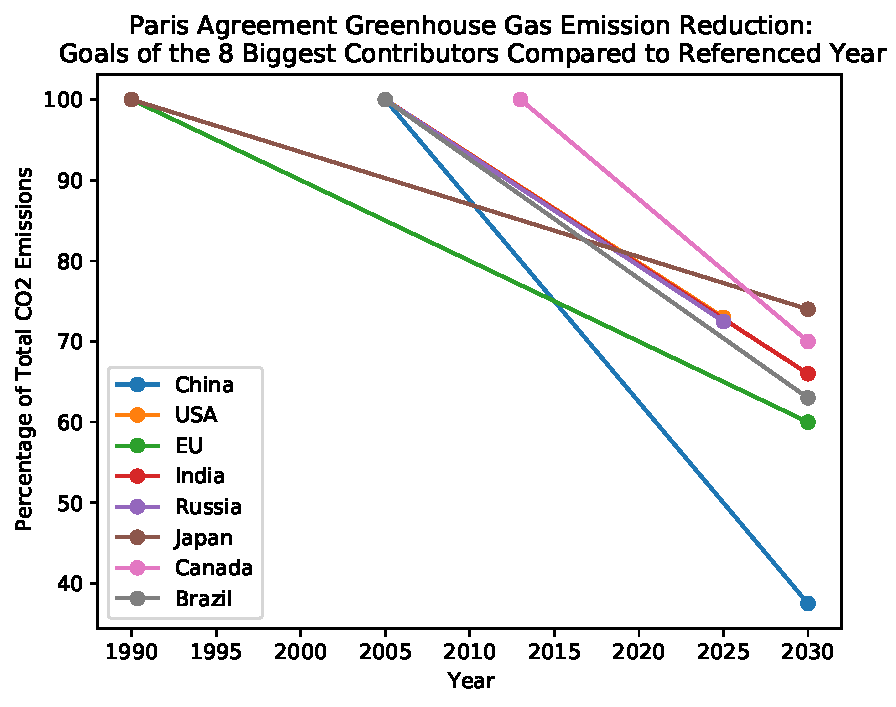
\includegraphics[width=0.8\textwidth]{co2goals/co2goals_lines.pdf}
%			\caption{Line plot for each country's goal compared to the reference year. The $y$-axis represents the greenhouse gas emissions of each country in percent, the $x$-axis the year. Each line starts at (referred  year, 1) and ends at (\(1-\)goal, targeted year). The slopes thus represent the rate of reduction per year in \%/year. This plot does not state anything about absolute data or the contribution of the countries to global greenhouse gas emissions however.}
%			\label{fig:co2goals_line}
%		\end{subfigure}\hfill
%		\begin{subfigure}[b]{0.49\linewidth}
%			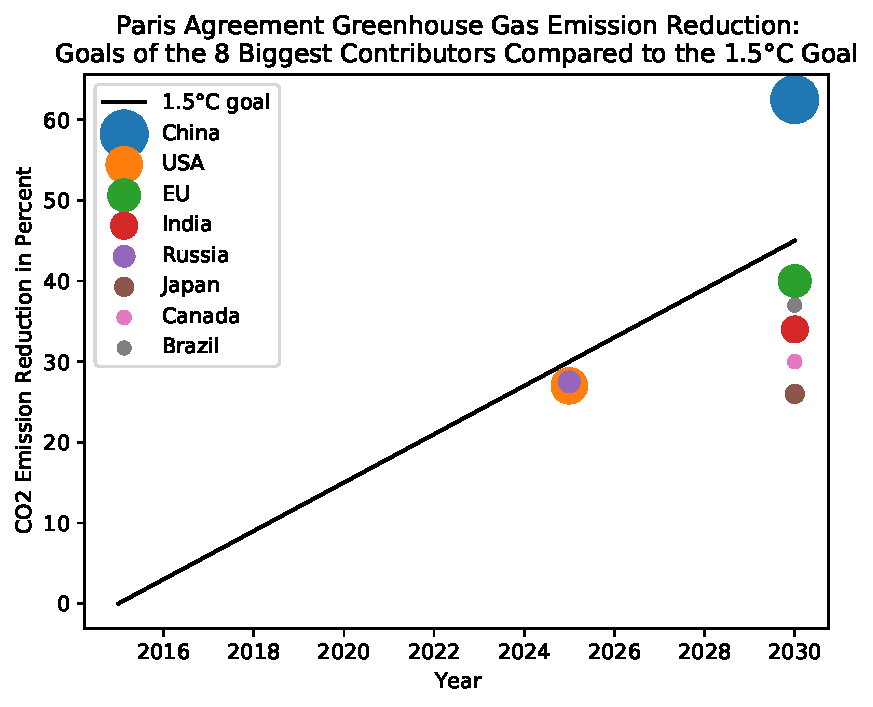
\includegraphics[width=0.8\textwidth]{co2goals/co2goals_bubbles.pdf}
%			\caption{Bubble plot that visualizes how ambitious each country is. The $y$-axis represents the greenhouse gas emission reduction goal in percent, the $x$-axis the year. The size of each bubble corresponds to its share in global greenhouse gas emissions. The black line gives the necessary emission reductions to reach the \SI{1.5}{\degreeCelsius} goal.}
%			\label{fig:co2goals_bubble}
%		\end{subfigure}
%	\end{center}
%\end{figure}









\begin{figure}[htb]
	\begin{center}
		\begin{subfigure}[b]{0.49\linewidth}
			\centering
			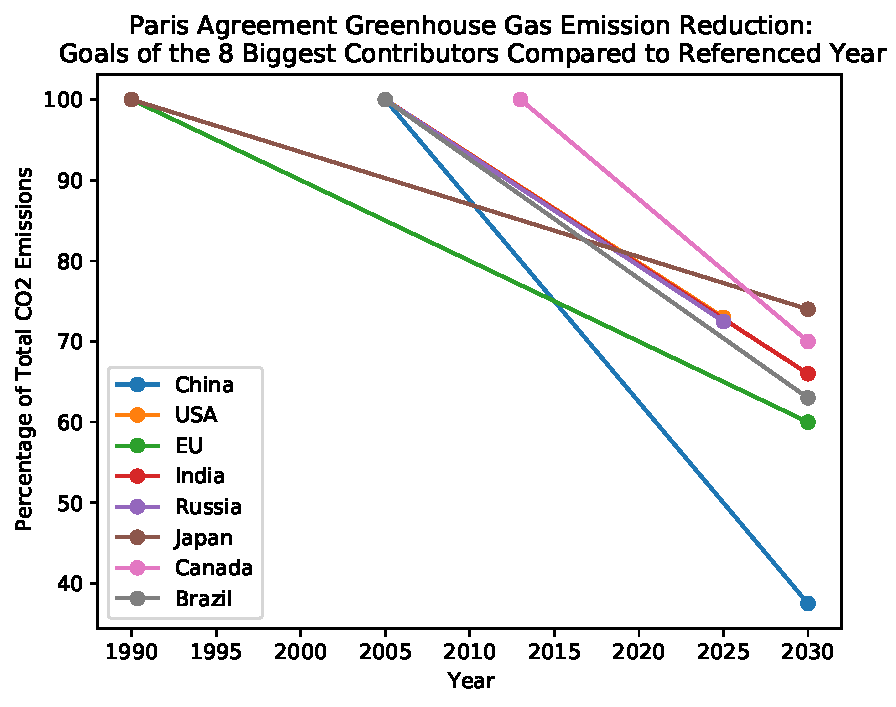
\includegraphics[width=0.8\textwidth]{co2goals/co2goals_lines.pdf}
			\caption{}
			\label{fig:co2goals_line}
		\end{subfigure}\hfill
		\begin{subfigure}[b]{0.49\linewidth}
			\centering
			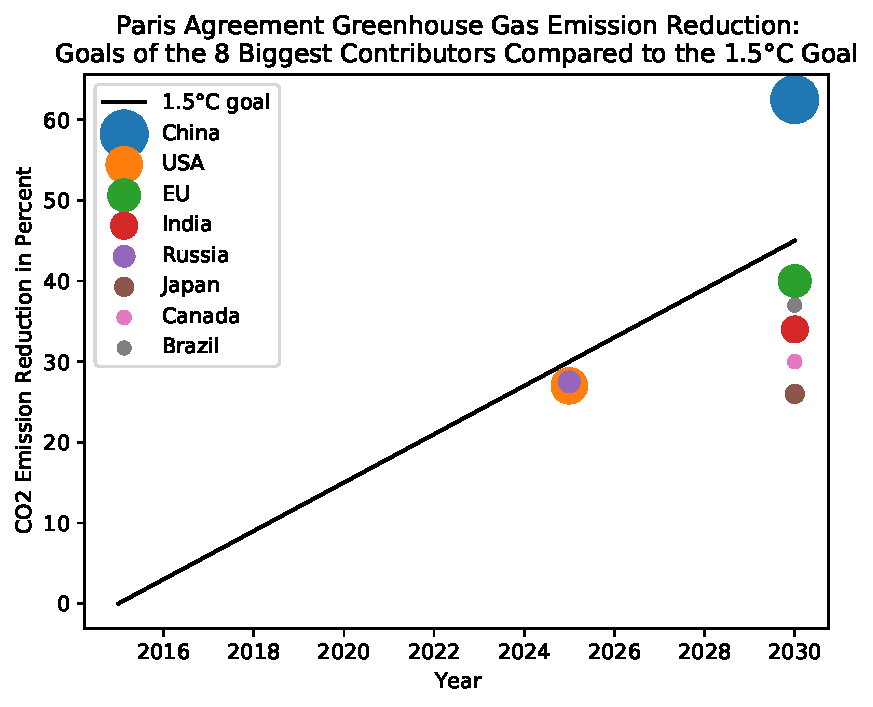
\includegraphics[width=0.8\textwidth]{co2goals/co2goals_bubbles.pdf}
			\caption{}
			\label{fig:co2goals_bubble}
		\end{subfigure}
		\caption{\textbf{a.} Line plot for each country's goal compared to the reference year. The $y$-axis represents the greenhouse gas emissions of each country in percent, the $x$-axis the year. Each line starts at (referred  year, 1) and ends at (\(1-\)goal, targeted year). The slopes thus represent the rate of reduction per year in \%/year. This plot does not state anything about absolute data or the contribution of the countries to global greenhouse gas emissions however.
			\textbf{b.}	Bubble plot that visualizes how ambitious each country is. The $y$-axis represents the greenhouse gas emission reduction goal in percent, the $x$-axis the year. The size of each bubble corresponds to its share in global greenhouse gas emissions. The black line gives the necessary emission reductions to reach the \SI{1.5}{\degreeCelsius} goal.}
	\end{center}
\end{figure}










\subsection{Usage of Emission Reduction Goals Data}
The data we gathered is crucial for our project. With the data, we can compare the greenhouse gas reduction due to the COVID-19 pandemic with the actual goals each country set for itself. From that, we can quantify how much this reduction contributes to the goals. As we have data of the emitters accounting for over two thirds of global greenhouse gas emissions, we not only see how COVID-19 related emission reductions help some individual countries to reach their goals but also see its global impact. For this reason, the data about emission reduction goals -- along with COVID-19 and greenhouse gas emission data -- counts to the most important data sets of our project.






%for \SI{1.5}{\degreeCelsius}, we need to cut emissions by 45\% by 2030\footnote{see \url{https://www.scientificamerican.com/article/global-promises-to-reduce-co2-are-falling-short-of-1-5-degree-c-warming-goal/}}.


% What different sources did you look into and what are their pro's and con's. Are there alternatives?, check

% What did you do to prepare the dataset: cleaning, aligning, quality checking, balancing, etc.), check

% include plots, check

% describe them, check

% Check if collected data is useful, check

% Provide an assessment if you expect the data to be relevant for your project. In what way?, check
